\documentclass[usenames, dvipsnames]{article}      % article class
\usepackage[utf8]{inputenc}
\newcommand{\mytitle}{Hybrid tropical cyclones hazard modelling, focusing on storm surges on the US East coast}
\newcommand{\penname}{Simon~Thomas}
\usepackage{moreverb} 
\usepackage{Theme/mystyle}
\usepackage{Theme/linkcolors}
\usepackage{Theme/referencing}
\usepackage{Theme/globals}
\graphicspath{{images/}{../images/}}
\addbibresource{references/generic_references.bib}
\addbibresource{references/references.bib}
\addbibresource{references/fluid_dynamics.bib}
\addbibresource{references/machine_learning.bib}
\addbibresource{references/global_warming.bib}
\addbibresource{references/programming.bib}
\addbibresource{references/surge.bib}
\addbibresource{references/tebbutt.bib}
\addbibresource{references/taleb.bib}
\addbibresource{references/evt.bib}
\addbibresource{references/cyclone.bib}
\addbibresource{references/meteorology.bib}

% \RequirePackage{fancyhdr}    % use fancyhdr to customize hdrs & ftrs
\RequirePackage[margin=2.5cm, headheight=15pt, includeheadfoot]{geometry}
\renewcommand{\headrulewidth}{0pt}   % suppress rule across top(fancyhdr default)
\setlength\headheight{26pt} %% just to make a warning go away.
\rhead{\thepage}  % right head page number.
% page number on right head
\lfoot{\penname}  % left foot author.
\cfoot{}
\rfoot{}
\pagestyle{fancy}  % use fancyhdr style

\RequirePackage[linesnumbered,ruled,vlined]{algorithm2e}

\usepackage{array}
\newcolumntype{L}[1]{>{\raggedright\let\newline\\\arraybackslash\hspace{0pt}}m{#1}}

\title{\vspace*{-100pt}\textbf{\mytitle}\vspace{-0pt}}
\date{\today}
\author{\penname}

\usepackage[fontsize=12pt]{fontsize}
\begin{document}
\maketitle
\begin{abstract}
    
This document sets out some ideas for a PhD project at the AI4ER CDT program.  I want to focus on the hazards 
from tropical cyclones because they are substantial, 
and the basics of tropical cyclones can be understood by quite simple theory.
Data driven approaches are limited by the 
lack of long period high quality data:
observations are only available for limited
timescales and locations; models are limited by
time/space resolution, total length of model runs, and bias.
It is likely that a hybrid approach that incorporates
physical knowledge and data will be the most fruitful.

\end{abstract}

\subsection*{Motivation}
Storm surges are coastal sea levels which far exceed those
expected given the tide.
They are caused by tropical cyclones
(TCs) and extratropical cyclones (ECs).
TCs draw their kinetic energy from the thermodynamic disequilibrium between
the tropical sea surface and the
troposphere~\cite{emanuel1986air, emanuel1987dependence},
whereas ECs draw theirs from the
polewards temperature
gradient~\cite{lorenz1960energy, holton2004introduction} at higher latitudes.
Because they have lower central pressures and sustain greater winds,
TCs create more dangerous storm surges~\cite{emanuel2005divine},
and so ECs will be ignored.

TCs have historically been the
world's largest physical hazard~\cite{shultz2005epidemiology},
for economic damage,
and specifically TC storm surges for lives lost~\cite{emanuel2005divine,
shultz2005epidemiology, zhang2009tropical}.
This hazard is increasing as more people live on vulnerable coastlines
in substandard buildings~\cite{emanuel2005divine}.
Anthropogenic climate change is expected to exacerbate this,
as it begins to increase the maximum TC intensity\footnote{
However the uptick in TCs is not currently above
 natural variability~\cite{mendelsohn2012impact}.}
~\cite{
emanuel2008hurricanes,emanuel2017will, nordhaus2010},
increased range~\cite{emanuel2008hurricanes, emanuel2017will, fedorov2010tropical}.
and to sea level rise placing more areas at risk~\cite{SROCC}.


It is necessary to quantify how this hazard will change
so that the public can act with foresight.
Others have already applied machine learning (ML) techniques to this
end~\cite{kulp2019new, kulp2018coastaldem, tadesse2020data}.
The motivation for hybrid physical/ML modelling is simple:
an algorithm that does not respect physical laws
may fit the data well
it is more likely to generalise poorly to unseen data~\cite{beucler2019achieving}.

\subsection*{My previous work}

It is an open question whether there are ways of summarising the characteristics of a tropical cyclone and the coastline so that good statistical models can be built to assess their impact, as a more efficient alternative to high resolution 3D modelling. Particular features, such as the distance to the 30m contour have been used as informative statistical features for hazard models (see e.g. [A]). My MSci Project \url{https://bit.ly/msci-report}, \url{https://bit.ly/msci-summary} showed that you can predict the responsiveness of a coastline to a wind stress fairly well with a simple physical model in figure~\ref{fig:responsiveness}.

\begin{figure}
    \centering
    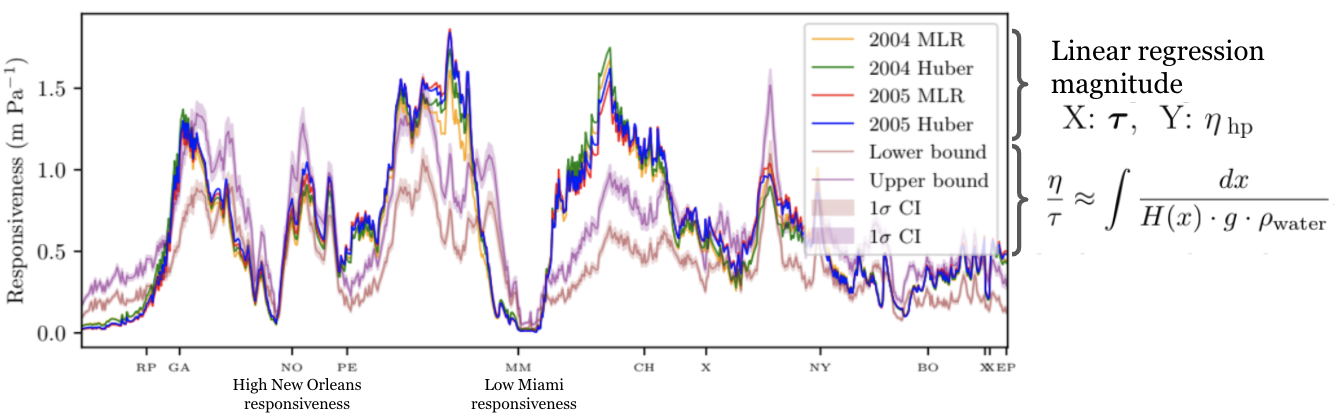
\includegraphics[width=1.1\linewidth]{img.png}
    \caption{The simple responsiveness metric from my MSci thesis.}
    \label{fig:responsiveness}
\end{figure}

\subsection*{Initial PhD project direction}

This metric captured the broad trends seen in the model output. As a possible improvement, we propose to develop better feature engineering to incorporate elements such as the convexity of the coast, in a model similar to Chavas et al. [A]. Talea Mayo (Emory University) has offered to provide an initial storm surge dataset that was produced in collaboration with Ning Lin [B, C, D], and this could provide an initial dataset to address the scientific question:

\subsection*{Potential PhD project questions:}

\begin{itemize}
    \item Are there metrics that can summarise the bathymetry’s impact on the size of the storm surge from a given tropical cyclone?

    \item More generally, is it possible to build a statistical or machine learning type model to connect a variety of features (e.g. bathymetry, local winds) to storm surge risk?

    \item Even more generally, can we extend this framework to other forms of risk (e.g. wind damage)?
\end{itemize}

\subsection*{Additional Papers:}


[A] Chavas, Daniel, et al. ``US hurricanes and economic damage: Extreme value perspective.'' Natural Hazards Review 14.4 (2013): 237-246.

[B] Marsooli, R., Lin, N., Emanuel, K. and Feng, K., 2019. Climate change exacerbates hurricane flood hazards along US Atlantic and Gulf Coasts in spatially varying patterns. Nature communications, 10(1), pp. 1-9.

[C] Marsooli, R. and Lin, N., 2018. Numerical modeling of historical storm tides and waves and their interactions along the US East and Gulf Coasts. Journal of Geophysical Research: Oceans, 123(5), pp.3844-3874.

[D] Lin N, Emmanuel K, 2016. Grey Swan tropical cyclones


\printbibliography
\end{document}
